\section{Implementation}
\label{sec-impl}

In \S \ref{sec-methods}, the strategies and interfaces that \Cyclus uses to 
simplify archetype development were presented. These represent notions about
the amount of information and prior knowledge that the archetype developer 
must have in order to write archetypes.  If a particular strategy 
decreases the knowledge required by archetype developers then it is considered
beneficial to implement.  

However, methods that are more intuitive for new users to understand are often
proportionately more difficult to implement. For example, playing or mastering 
the game \emph{tic-tac-toe} is a vastly different effort than
designing the game in the first place.  
A sublime interface belies 
herculean effort. This section describes the infrastructure of
current \cyclus archetype development.  This is relevant to other fuel 
cycle simulators that wish to adopt the same strategies that \cyclus 
implements. In particular, the implementation of the \cyclus preprocessor, 
the type system, input file validation, and metadata annotations will all 
be covered here.

\subsection{The \Cyclus Preprocessor}

The \cyclus preprocessor, \cycpp, is responsible for all metadata collection and 
code generation for archetypes. It is implemented as a small Python utility 
that is currently less than 2000 lines in a single file.  It has no dependencies other 
than the Python standard library \cite{lutz2010programming}. It is thus light-weight enough to move around 
between code projects, if needed. For the scale of its responsibility, \cycpp
is extremely efficient. 

The preprocessor implements the three passes detailed in \S\ref{subsec-ppgc}:
normalization via standard \code{cpp}, state variable annotation accumulation, and code 
generation. The \cycpp tool must be run on all C++ header and source files that
contain archetype code and the \code{#pragma cyclus} directives. Running \cycpp
on files without such directives will result in exactly the 
original file. The first \cycpp
pass, running the C preprocessor over these files, is a trivial subprocess 
spawn. Importantly, \cycpp was ensured to detect the
same include, macro definitions, and macro un-definitions that actual compilation 
of the source code includes.

The second pass, state accumulation, represents half of the work that \cycpp performs.
The results from pass one are fed into this pass and scoured for 
potentially relevant information about the archetypes present in the file. 
Thus, state accumulation 
may be thought of as a traditional parser that transforms tokens (lines of the 
C++ file) into a more meaningful in-memory data structure. As a parser, pass two 
may be implemented as a \emph{state machine}
\cite{mertz2003text,wagner2006modeling}.

Pass two is represented in \cycpp by the \code{StateAccumulator} class,  a
state machine that compares the output lines from the C preprocessor against a series of \emph{filters}.  If a line matches the expected structure 
for a filter, then the filter executes a \emph{transformation} function on the 
line and no further filters are executed. If the line does not match any 
filters, then the line is allowed to pass through the \code{StateAccumulator}.  
The filter-transformation sequence can be thought of in analogy to a sphere of 
a given radius (a line of code) attempting to pass through concentric windows 
(the filters) of decreasing aperture, as illustrated in Figure \ref{filter-analogy}. 
This first window where the sphere stops 
represents the transformation that is executed.  This sphere is allowed to move 
through the system without being stopped.

\begin{figure}[htbc]
\centering
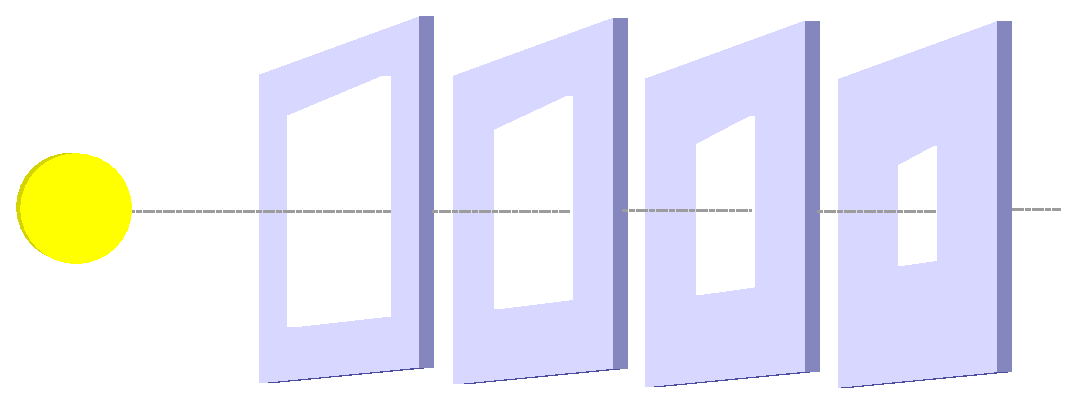
\includegraphics[width=0.8\textwidth]{filter-analogy.eps}
\caption{The \code{StateAccumulator} class passes lines of C++ code through 
a series of filters, each of which may transform the information heretofore gathered
by previous filters. 
This may be thought of analogous to a spheres of various radii traversing 
concentric windows.  The spheres, or lines of code, stop when they cannot pass a  
window, or filter. This triggers the execution of the transformation function of just 
that filter.}
\label{filter-analogy}
\end{figure}

The filters implemented for pass two of \cycpp are described in Table \ref{pass2-filters}, 
in order of decreasing precedence. The most important of these filters implement 
the \code{#pragma cyclus} directives that the archetype uses to communicate
with the preprocessor.  The pragma filters typically modify attributes of
the \code{StateAccumulator}, such as the \code{context}, the \code{execns} 
(or \emph{execution namespace}), the \code{aliases} set, and the \code{namespaces}. 
These represent the classes, types, aliases, and other information that defines
the scope of the C++ code. Such information is necessary 
for accurately representing archetypes and their state variables. 

Most pass two filters that do not implement a preprocessor directive instead
aggregate information about the available types. The \code{VarDeclarationFilter} has
the important job of determining the C++ type of state variables from the 
member variable declaration on the archetype class. However, the C++ type system 
is complex and allows for a number of programmer modifications prior 
to the type declarations:
\begin{itemize}
    \item types may be aliased to any number of alternative names, 
    \item template types are white-space insensitive, 
    \item scoping rules apply to new type names, and 
    \item other issues must be resolved to accurately and uniquely represent a C++ type. 
\end{itemize}
This requires that \cycpp implement relevant type handling
simply to correctly spell the canonical type name. 
Thus the \code{StateAccumulator} class acts as its own type system and
returns the canonical form of any type it knows about at all points during 
pass two of \cycpp.

\begin{table}
\caption{\cyclus Preprocessor Pass 2 Filters (Higher order filters have 
         lower execution precedence)}
\begin{tabular}[htb]{|p{0.05\linewidth}|p{0.33\linewidth}|p{0.6\linewidth}|}
\hline
\textbf{order} & \textbf{filter} & \textbf{description} \\
\hline
1  & \code{ClassAndSuperclassFilter} & Accumulates the class name from a class 
                                       declaration. Also stores the names of the 
                                       superclasses from the declaration.\\ 
\hline
2  & \code{AccessFilter} & Sets the current access control level:
                           \code{public}, \code{private}, or \code{protected}.\\
\hline
3  & \code{ExecFilter} & Implements the \code{#pragma cyclus exec <code>} directive
                         that allows for the execution of arbitrary Python code.
                         The results of this code are added to the context that 
                         evaluates other \cycpp directives.\\ 
\hline
4  & \code{UsingNamespaceFilter} & Adds and removes a namespace from the 
                                   current scope via the C++ \code{using namespace}
                                   statement.\\ 
\hline
5  & \code{NamespaceAliasFilter} & Implements namespace aliasing in the current 
                                   scope.\\ 
\hline
6  & \code{NamespaceFilter} & Sets and reverts a new namespace scope.\\ 
\hline
7  & \code{TypedefFilter} & Adds a type alias to the current scope via the 
                            C++ \code{typedef} statement.\\ 
\hline
8  & \code{UsingFilter} & Removes scope from a type by adding an alias in the 
                          current scope via the C++ \code{using} statement.\\ 
\hline
9  & \code{LinemarkerFilter} & Interprets \code{cpp} linemarker directives in order
                               to produce more useful debugging information in 
                               \cycpp.\\ 
\hline
10 & \code{NoteDecorationFilter} & Implements the \cycpp \code{#pragma cyclus note <dict>}
                                   directive by evaluating the contents of 
                                   \code{<dict>} and adding them to the archetype 
                                   annotations.\\ 
\hline
11 & \code{VarDecorationFilter} & Implements the \cycpp \code{#pragma cyclus var <dict>}
                                  directive for state variable annotations
                                  by evaluating the contents of \code{<dict>} in the current 
                                  context and queuing  them for the 
                                  next state variable declaration.\\ 
\hline
12 & \code{VarDeclarationFilter} & State variable declaration. Applies the results 
                                   of the immediately prior \code{VarDecorationFilter}
                                   as the state variable annotations. Furthermore, 
                                   this filter parses out the name of the 
                                   state variable, its index with respect to other 
                                   state variables on this class, and resolves its
                                   C++ type into an unambiguous form.\\ 
\hline
13 & \code{PragmaCyclusErrorFilter} & Throws errors if \code{#pragma cyclus} 
                                      directive is incorrectly implemented.
                                      This moves errors from happening at compile 
                                      or run time to \cycpp.\\
\hline
\end{tabular}
\label{pass2-filters}
\end{table}

In \cycpp, the only relevant type information is the name.  The concrete size in bits
of a type and the operations that are available for that type are not directly 
relevant. This is because the primary purpose of the type of a state variable is
to be able to fill in the relevant value in the third pass of code generation. Further 
reflection is not used by \cycpp itself, so the canonical spelling of the type 
name is the only information used.  

The canonical form of a type has the following spelling rules:
\begin{itemize}
    \item Primitive types (\code{int}, \code{double}, \code{std::string}, etc.) 
          and classes (\code{cyclus::Blob}, etc.) are spelled with strings 
          of the names.
    \item Template types (\code{std::vector}, \code{std::map}, etc.) are spelled 
          with lists of length of the number of template parameters plus one.
          The first element of the list is a string that represents the 
          template type (e.g. \code{std::pair}). The remaining elements of 
          the list represent the template parameter types, in order, and may 
          be either strings or lists.  For example, the type 
          \code{std::map<int, std::vector<double>>} would have the canonical form 
          of \code{['std::map', 'int' ['vector', 'double']]}.
    \item All namespaces must be included in the type name.
    \item Pointer and reference types are not allowed because these may not be 
          represented in the database.
\end{itemize}
The above rules create an accurate and language-independent
mechanism for spelling C++ types, including templates. The preprocessor is aware
of the following types that may be present in a \cyclus database in various 
combinations:
\begin{itemize}
    \item \textbf{Primitives:} \code{bool}, \code{int}, \code{float}, \code{double}, 
                               \code{std::string}
    \item \textbf{Known Classes:} \code{cyclus::Blob}, \code{boost::uuids::uuid}, 
                                  \code{cyclus::toolkit::ResourceBuff}
    \item \textbf{Templates:} \code{std::vector}, \code{std::set}, \code{std::list}, 
                              \code{std::pair}, \code{std::map}
\end{itemize}

Resolving a canonical type name is necessarily a recursive process.
This is because aliases may point to other aliases --- not just primitive type names.
Thus to resolve an alias, one must walk through an arbitrarily deep graph of aliases 
to find the associated primitive.  For example, given that \code{myfloat} points 
to \code{float} (the primitive) and \code{mynumber} points to \code{myfloat}, 
if a state variable was declared as \code{myfloat} only one alias lookup would
be required whereas two would be required
if it was declared as \code{mynumber}. The canonical
form for all \code{float}, \code{myfloat}, and \code{mynumber} would all be 
\code{float}.  This is what \cycpp should record.  Templates must recursively 
determine the template type name and the types of all template parameters.
The canonical form of a type must be automatically computed to avoid an
entire class of typographic errors by the archetype developers.

Aside from the type system semantics, pass two represents a relatively straightforward
process of building up archetype information for later use. The first instance
of later use occurs during pass three of \cycpp,
code generation.  Conceptually, 
pass three is a more complex process than pass two because it must implement 
all of the member functions in Listing \ref{req-api}. In practice however, the body 
of each of these member functions follows its own pattern with respect to the 
state variables. Therefore, implementing pass three is significantly easier.

Much like pass two, pass three is also a state machine. The class that implements it is 
called \code{CodeGenerator} and the filters within this class implement 
the corresponding code generation routines.  While the \code{CodeGenerator}  does 
reuse some meta-data accumulation filters, it largely relies on the results of 
pass two for archetype and state variable information.  The only data that cannot be 
reused and is recomputed is that which pertains to the scope of each line of C++ code.

Pass three traverses all lines of the source code for a third time.
On this pass, the \code{CodeGenerator} will replace certain \code{#pragma cyclus}
directives with the generated implementations.  Pass three may act on the output of
\code{cpp}, the results of pass one.  However, it is more common for this 
to act on the original source and header files.  This requires that the 
archetype developer write in mostly normative C++ and not abuse the C
preprocessor,
avoiding double include errors and other downstream issues with 
compilation. The results of pass three, therefore, are a new version of the archetype
source code that differs only in that it contains automatically implemented 
member functions.

Table \ref{pass3-filters} displays the filters that the \code{CodeGenerator} 
employs in order of precedence. These filters overlap somewhat with
those of the \code{StateAccumulator}. This enables the efficient reuse
of filters between state machines.

\begin{table}
\caption{\cyclus Preprocessor Pass 3 Filters, higher order filters have 
         lower execution precedence.}
\begin{tabular}[htb]{|p{0.05\linewidth}|p{0.33\linewidth}|p{0.6\linewidth}|}
\hline
\textbf{order} & \textbf{filter} & \textbf{description} \\
\hline
1  & \code{InitFromCopyFilter} & Implements code generation for copy-constructor-like 
                                 \code{InitFrom()} member function. This may be called
                                 with the 
                        \code{#pragma cyclus [def\|decl\|impl] initfromcopy [classname]}
                                 directive.\\
\hline
2  & \code{InitFromDbFilter} & Implements code generation for database constructor 
                               \code{InitFrom()} member function. This may be called
                               with the 
                        \code{#pragma cyclus [def\|decl\|impl] initfromdb [classname]}
                               directive.\\
\hline
3  & \code{InfileToDbFilter} & Implements code generation for the \code{InfileToDb()} 
                               member function that converts an input file into its 
                               database representation. This may be called with the 
                        \code{#pragma cyclus [def\|decl\|impl] infiletodb [classname]}
                               directive.\\
\hline
4  & \code{CloneFilter} & Implements code generation for the \code{Clone()} member
                          function that clones prototypes. This may be called
                          with the 
                        \code{#pragma cyclus [def\|decl\|impl] clone [classname]}
                          directive.\\
\hline
5  & \code{SchemaFilter} & Implements code generation for the \code{schema()} member
                           function that returns the \gls{RNG} schema of the archetype
                           for input file validation. This may be called with the 
                        \code{#pragma cyclus [def\|decl\|impl] schema [classname]}
                           directive.\\
\hline
6  & \code{AnnotationsFilter} & Implements code generation for the \code{annotations()} 
                                member function that returns the archetype metadata
                                that was compiled during \cycpp pass two.
                                This may be called with the 
                        \code{#pragma cyclus [def\|decl\|impl] annotations [classname]}
                                directive.\\
\hline
7  & \code{InitInvFilter} & Implements code generation for the \code{InitInv()} 
                            member function that sets the initial resource inventories 
                            of the agent. This may be called with the 
                        \code{#pragma cyclus [def\|decl\|impl] initinv [classname]}
                            directive.\\
\hline
8  & \code{SnapshotInvFilter} & Implements code generation for the \code{SnapshotInv()} 
                                member function that writes inventories to the 
                                database. This may be called with the 
                        \code{#pragma cyclus [def\|decl\|impl] snapshotinv [classname]}
                                directive.\\
\hline
9  & \code{SnapshotFilter} & Implements code generation for the \code{Snapshot()} 
                             member function that writes state variables to the
                             database. This may be called with the 
                        \code{#pragma cyclus [def\|decl\|impl] snapshot [classname]}
                             directive.\\
\hline
10 & \code{ClassFilter} & Sets the current class name and scope.\\
\hline
11 & \code{AccessFilter} & Sets the current access control level, either 
                           \code{public}, \code{private}, or \code{protected}.\\
\hline
12 & \code{NamespaceAliasFilter} & Implements namespace aliasing in the current 
                                   scope.\\ 
\hline
13 & \code{NamespaceFilter} & Sets and reverts a new namepsace scope.\\ 
\hline
\end{tabular}
\label{pass3-filters}
\end{table}

\begin{table}
\caption{\cyclus Preprocessor Pass 3 Filters (part 2).}
\begin{tabular}[htb]{|p{0.05\linewidth}|p{0.33\linewidth}|p{0.6\linewidth}|}
\hline
\textbf{order} & \textbf{filter} & \textbf{description} \\
\hline
14 & \code{VarDecorationFilter} & Implements the \cycpp \code{#pragma cyclus var <dict>}
                                  directive for state variable annotations 
                                  by evaluating the contents of \code{<dict>} in the current 
                                  context and queuing them for the 
                                  next state variable declaration.\\ 
\hline
15 & \code{VarDeclarationFilter} & State variable declaration. Applies the results 
                                   of the immediately prior \code{VarDecorationFilter}
                                   as the state variable annotations. Furthermore, 
                                   this filter parses out the name of the 
                                   state variable, its index with respect to other 
                                   state variables on this class, and resolves its
                                   C++ type into an unambiguous form.\\ 
\hline
16 & \code{LinemarkerFilter} & Interprets \code{cpp} linemarker directives in order
                               to produce more useful debugging information in 
                               \cycpp.\\ 
\hline
17 & \code{DefaultPragmaFilter} & Implements the default code generation directive,
                                  \code{#pragma cyclus [def\|decl\|impl]}. This 
                                  calls the other code generation
                                  filters to obtain member function implementations.\\
\hline
18 & \code{PragmaCyclusErrorFilter} & Throws errors if \code{#pragma cyclus} 
                                      directive is incorrectly implemented.
                                      This moves errors from happening at compile 
                                      or run time to \cycpp.\\
\hline
\end{tabular}
\label{pass3-filters-2}
\end{table}

When all of the pieces of \cycpp are brought together, the benefits scale as the 
number of state variables times the number of code generated member functions 
(currently nine). This implies roughly an order of magnitude savings on the number of 
lines that an archetype developer must write per state variable. Moreover, 
exponential savings come from the fact that the archetype developers do not need
to understand either the \cyclus interface nor the extra lines that they do not have to write.
Even for a developer who knows the \cyclus
interface completely, there is still almost ten times less to write. Consider 
again the simple \code{Reactor} example presented in Listing \ref{rx-eg}.  These twelve 
lines of code are transformed into 112 lines by \cycpp, the results of which
are shown in Listing \ref{rx-eg-cycpp}. 

\begin{lstlisting}[caption={Simple Reactor Archetype After Preprocessing with \cycpp, 
                            line marker directives have been removed for space}, 
                   label=rx-eg-cycpp]
class Reactor : public cyclus::Facility {
 public:
  Reactor (cyclus::Context* ctx) {};
  virtual ~Reactor() {};

  virtual void InitFrom(Reactor* m) {
    flux = m->flux;
    power = m->power;
    shutdown = m->shutdown;
  };

  virtual void InitFrom(cyclus::QueryableBackend* b) {
    cyclus::QueryResult qr = b->Query("Info", NULL);
    flux = qr.GetVal<double>("flux");
    power = qr.GetVal<float>("power");
    shutdown = qr.GetVal<bool>("shutdown");
  };

  virtual void InfileToDb(cyclus::InfileTree* tree, cyclus::DbInit di) {
    tree = tree->SubTree("config/*");
    cyclus::InfileTree* sub;
    int i;
    int n;
    flux = cyclus::OptionalQuery<double>(tree, "flux", 4e+14);
    power = cyclus::OptionalQuery<float>(tree, "power", 1000);
    shutdown = cyclus::Query<bool>(tree, "shutdown");
    di.NewDatum("Info")
    ->AddVal("flux", flux)
    ->AddVal("power", power)
    ->AddVal("shutdown", shutdown)
    ->Record();
  };

  virtual cyclus::Agent* Clone() {
    Reactor* m = new Reactor(context());
    m->InitFrom(this);
    return m;
  };

  virtual std::string schema() {
    return ""
      "<interleave>\n"
      "<optional>\n"
      "    <element name=\"flux\">\n"
      "        <data type=\"double\" />\n"
      "    </element>\n"
      "</optional>\n"
      "<optional>\n"
      "    <element name=\"power\">\n"
      "        <data type=\"float\" />\n"
      "    </element>\n"
      "</optional>\n"
      "<element name=\"shutdown\">\n"
      "    <data type=\"boolean\" />\n"
      "</element>\n"
      "</interleave>\n"
      ;
  };

  virtual Json::Value annotations() {
    Json::Value root;
    Json::Reader reader;
    bool parsed_ok = reader.parse(
      "{\"name\":\"Reactor\",\"entity\":\"unknown\",\"parents\":[],"
      "\"all_parents\":[],\"vars\":{\"flux\":{\"default\":4000000"
      "00000000.0,\"units\":\"n/cm2/2\",\"type\":\"double\",\"inde"
      "x\":0},\"power\":{\"default\":1000,\"units\":\"MWe\",\"type\""
      ":\"float\",\"index\":1},\"shutdown\":{\"doc\":\"Are we "
      "operating?\",\"type\":\"bool\",\"index\":2}}}", root);
    if (!parsed_ok) {
      throw cyclus::ValueError("failed to parse annotations for Reactor.");
    }
    return root;
  };

  virtual void InitInv(cyclus::Inventories& inv) {
  };

  virtual cyclus::Inventories SnapshotInv() {
    cyclus::Inventories invs;
    return invs;
  };

  virtual void Snapshot(cyclus::DbInit di) {
    di.NewDatum("Info")
    ->AddVal("flux", flux)
    ->AddVal("power", power)
    ->AddVal("shutdown", shutdown)
    ->Record();
  };

 private:
  #pragma cyclus var {'default': 4e14, 'units': 'n/cm2/2'}
  double flux;

  #pragma cyclus var {'default': 1000, 'units': 'MWe'}
  float power;

  #pragma cyclus var {'doc': 'Are we operating?'}
  bool shutdown;
};
\end{lstlisting}

Of course, archetypes may be much more complex than the \code{Reactor} example.
This archetype does not participate in resource exchange, take advantage of 
the reflection features, use more advanced annotation features, or have more than 
a handful of state variables.  Yet, even here, the value of a code generating
preprocessor is readily apparent.

\subsection{Database Backends \& Types}

\Cyclus transparently supports a potentially limitless number of different database 
backends. Currently, two reference backends exist: \gls{SQLite} \cite{owens2006definitive} 
and \gls{HDF5} \cite{folk2011overview}. These two represent relational and hierarchical 
databases, respectively, and have different underlying design philosophies.
Future formats that could be supported include plain text 
\gls{CSV} files or \gls{JSON}.  Given the wide range of potential uses cases, \cyclus must be able 
to execute based on only the feature set that is common among these formats.
Features that are not available in a single format must either be provided by \cyclus 
itself or become optional in the backend interface.

The type system and reflection provided by \cycpp 
allow archetypes to represent themselves in the database. Though this 
reflection can be taken advantage of and used elsewhere, it was initially
implemented because of the need to restart a simulation.
The database model extends well beyond the needs of the archetypes alone by 
serving as the fundamental on-disk representation for all \cyclus input and output.

\Cyclus databases follow these fundamental abstractions:
\begin{itemize}
    \item All data are stored in tables with named columns,
    \item Tables live in a flat hierarchy,
    \item Columns may have any type described by the \cyclus type system, and
    \item All tables must have a \code{SimId} column which uniquely and 
          universally identifies the simulation.
\end{itemize}
Therefore, common databases notions such as the shape of a column, raw arrays, or
queryability must be optional, omitted, or implemented inside the backend itself.
Queryability is the most important, and is available in both \gls{HDF5} and 
\gls{SQLite}. If a database format or its backend lacks 
queryability (such as \gls{CSV}), then it is impossible to start or restart a 
\cyclus simulation from simply this backend (though such a format may be used in 
conjunction with another queryable format). 

The database backends are deeply tied to the \cyclus type system. Types in \cyclus
are represented by unique integers that map to C++ types by the \code{enum} called \code{DbTypes}.
Simple types are represented by simple names: \code{float} becomes
\code{FLOAT}, which is assigned to 2. Container types, such as \code{vector},
are more complex in that each template specification (\code{vector<int>}) has
its own type in the \cyclus type system.  Containers are further delineated
as either fixed-length or \gls{VL}. Thus even the 
relatively simple C++ type \code{std::vector<int>} receives two entries in the 
\cyclus type system: \code{VECTOR_INT} and \code{VL_VECTOR_INT}, which are given 
the identifiers 10 and 11 and represent fixed- and variable-length versions, 
respectively.  Thus the number of types in the \cyclus type system is obtained as 
2 to the power of the \emph{rank} or the total number of variable length parameters, 
including nettings.
For example, the number of \cyclus types for \code{std::map<int, std::string>} is 
four (\code{MAP_INT_STRING}, \code{VL_MAP_INT_STRING}, \code{MAP_INT_VL_STRING}, 
\code{VL_MAP_INT_VL_STRING}) since both maps and strings may be variable length.
Table \ref{some-types} displays a sampling of types currently implemented in 
\cyclus.
Each backend determines which types it wishes to support, though this must extend 
to a relatively robust subset in order to run even simple simulations.

\begin{table}
\caption{Sample \cyclus Types}
\centering
\begin{tabular}[htb]{|c|l|l|c|}
\hline
\textbf{id} & \textbf{name} & \textbf{C++ type} & \textbf{rank} \\
\hline
0 & \code{BOOL} & \code{bool} & 0 \\
1 & \code{INT} & \code{int} & 0 \\
2 & \code{FLOAT} & \code{float} & 0 \\
3 & \code{DOUBLE} & \code{double} & 0 \\
4 & \code{STRING} & \code{std::string} & 1 \\
5 & \code{VL_STRING} & \code{std::string} & 1 \\
6 & \code{BLOB} & \code{cyclus::Blob} & 0 \\
7 & \code{UUID} & \code{boost::uuids::uuid} & 0 \\
8 & \code{VECTOR_BOOL} & \code{std::vector<bool>} & 1 \\
9 & \code{VL_VECTOR_BOOL} & \code{std::vector<bool>} & 1 \\
10 & \code{VECTOR_INT} & \code{std::vector<int>} & 1 \\
11 & \code{VL_VECTOR_INT} & \code{std::vector<int>} & 1 \\
 & $\cdots$ & $\cdots$ & \\
32 & \code{SET_STRING} & \code{std::set<std::string>} & 2 \\
33 & \code{VL_SET_STRING} & \code{std::set<std::string>} & 2 \\
34 & \code{SET_VL_STRING} & \code{std::set<std::string>} & 2 \\
35 & \code{VL_SET_VL_STRING} & \code{std::set<std::string>} & 2 \\
 & $\cdots$ & $\cdots$ & \\
42 & \code{LIST_INT} & \code{std::list<int>} & 1 \\
43 & \code{VL_LIST_INT} & \code{std::list<int>} & 1 \\
 & $\cdots$ & $\cdots$ & \\
57 & \code{PAIR_INT_INT} & \code{std::pair<int, int>} & 0 \\
 & $\cdots$ & $\cdots$ & \\
104 & \code{MAP_STRING_STRING} & \code{std::map<std::string, std::string>} & 3 \\
105 & \code{VL_MAP_STRING_STRING} & \code{std::map<std::string, std::string>} & 3 \\
106 & \code{MAP_STRING_VL_STRING} & \code{std::map<std::string, std::string>} & 3 \\
107 & \code{VL_MAP_STRING_VL_STRING} & \code{std::map<std::string, std::string>} & 3 \\
 & $\cdots$ & $\cdots$ & \\
120 & \code{MAP_VL_STRING_STRING} & \code{std::map<std::string, std::string>} & 3 \\
121 & \code{VL_MAP_VL_STRING_STRING} & \code{std::map<std::string, std::string>} & 3 \\
122 & \code{MAP_VL_STRING_VL_STRING} & \code{std::map<std::string, std::string>} & 3 \\
123 & \code{VL_MAP_VL_STRING_VL_STRING} & \code{std::map<std::string, std::string>} & 3 \\
 & $\cdots$ & $\cdots$ & \\
\hline
\end{tabular}
\label{some-types}
\end{table}

A key database-enabling feature of the \cyclus type system is that 
the values of all types must be directly \emph{hashable} using a cryptographic hash.
This directness implies that pointer and reference types are not allowed. For most 
database backends, indirection is not a supported feature. For those backends which 
do support indirection, such as \gls{HDF5} and its linking mechanism, there is not a 
clear translation from indirection in memory to indirection on disk.   
Requiring hashable data types avoids several classes of errors entirely.  

Hashability serves a dual role with respect to the backends. The first is that 
it provides a mechanism for uniquely identifying all elements of a type within 
reason. \Cyclus uses the standard \gls{SHA1} \cite{eastlake2001us} algorithm to compute 
hash values as 160-bit integer.  Thus for types with a fixed bit width less than 
160, such as \code{int} (typically 32-bits) or \code{double} (64-bits), every 
element is uniquely identifiable. For variable-length data types or very long types,
the probability of a hash collision is only $2^{-160}$, which is approximately 
equal to $10^{-48}$.  This is an astronomically small possibility, even over the 
course of billions of simulations.  Thus, backends may use the hash to automatically
de-duplicate data and store every unique value only once.

The second purpose for hashing is to allow backends to implement the storage 
of variable-length types as a \emph{bidirectional hash map} using the 
\gls{SHA1} as a key.  This data structure is an associative array in which the values are 
uniquely determined from the keys \emph{and} the keys are uniquely
determined from 
the values. Furthermore, in \cyclus, the keys of this data structure are simply the 
hashes themselves. This differs from a typical hash map (e.g. Python dictionaries) 
in that they only require that values may be determined from the keys and only the
keys must be unique.  With a bidirectional hash map, knowing either the key or the value
will grant one the value or the key, respectively.  The \gls{HDF5} backend takes advantage 
of this data structure to store variable-length data in a 5-dimensional sparse array.
The hash is chopped up into an array of five 32-bit unsigned integers that 
index into this sparse array. Then the hash is stored in the table and used to access 
the value in the corresponding sparse array for that type.  This creates an efficient 
mechanism for storing vast amounts of potentially redundant variable-length data in 
a manner that mirrors the column storage for primitive types (\code{bool}, \code{int}, 
etc.). Since the hash is itself the index into a sparse array, the overhead from 
this lookup is minimal as compared with other parts of backend infrastructure.

Archetype developers may create their own custom tables in the database as well.
This is done through using the backend interface directly in the archetype. 
Data that are fully dependent parameters of the archetype are not appropriate 
as state variables and thus should not be stored in this way.  Custom tables 
have the same restrictions as other parts of the database as well as 
the additional restriction that they cannot reuse the table names that 
\cyclus itself uses. Writing to such tables is reserved for
the kernel. 
Table \ref{std-tabs} shows the standard tables generated by \cyclus.
Distinct from the previously mentioned custom tables, the kernel will also produce 
tables whose names are based on the 
archetype specification for representing the archetype on disk.  These tables
are also reserved for the kernel alone. 

\begin{table}
\caption{Standard Tables Reserved by the \Cyclus Kernel, Columns given in order with 
names and types.}
\centering
\begin{tabular}[htb]{|llp{0.75\linewidth}|}
\hline
\textbf{name} & \textbf{type} & \textbf{description} \\
\hline
\multicolumn{3}{|p{0.95\linewidth}|}{\textbf{Resources Table:} 
Encodes a heritage tree for all resources. 
Because resources 
are tracked as immutable objects, every time a resource changes in the 
simulation (split, combined, transmuted, decayed, etc.), a new entry is added
to this table. If two resources are 
combined, then the new resource entry will have the identifiers of the 
other two in its ``Parent1'' and ``Parent2'' columns. 
The \code{Resources}
table does not encode any information about where a resource exists. This information 
can be inferred from the \code{ResCreators} and 
\code{Transactions} tables.}\\
& & \\
\code{SimId} & \code{UUID} & Simulation identifier \\
\code{ResourceId} & \code{INT} & The unique ID for this resource entry. \\
\code{ObjId} & \code{INT} & A resources object id (\code{obj_id}) as it existed 
                            during the simulation simulation.\\
\code{Type} & \code{VL_STRING} & One of ``Material'' or ``Product''. These two types 
                                 of resources have different internal state stored 
                                 in different tables. If the type is product, 
                                 then the internal state can be found in the 
                                 \code{Products} table. If it is material, 
                                 then it is in the \code{Compositions} table.\\
\code{TimeCreated} & \code{INT} & The simulation time step at which this resource 
                                  state came into existence.\\
\code{Quantity} & \code{DOUBLE} & Amount of the resource in ``kg'' for material 
                                  resources. Amount in terms of the specific quality 
                                  for product resources.\\
\code{Units} & \code{VL_STRING} & ``kg'' for all material resources, ``NONE'' for 
                                   product resources.\\
\code{QualId} & \code{INT} & Used to identify the corresponding internal-state 
                             entry (or entries) in the \code{Products} or 
                             \code{Compositions} table depending on the resource type.\\
\code{Parent1} & \code{INT} & If a resource was newly created, this is zero. If this 
                              resource came from transmutation, 
                              combining, splitting, or decay then this is the 
                              parent ResourceId.\\
\code{Parent2} & \code{INT} & If a resource was newly created, this is zero. If this 
                              resource came from transmutation, decay, 
                              or splitting, this is also zero. If the resource 
                              came from combining then this is the second 
                              parent's ResourceId.\\
\hline
\multicolumn{3}{|p{0.95\linewidth}|}{\textbf{Compositions Table:}
Stores compositions. A composition consists of one or more nuclides and their respective mass fractions. 
Each nuclide within a composition has its own row but the same \code{QualId}.}\\
& & \\
\code{SimId} & \code{UUID} & Simulation identifier \\
\code{QualId} & \code{INT} & Key to associate this composition with one or more 
                             entries in the \code{Resources} table.\\
\code{NucId} & \code{INT} & Nuclide identifier in zzzaaammmm form.\\
\code{MassFrac} & \code{DOUBLE} & Mass fraction for the nuclide in this composition.\\
\hline
\multicolumn{3}{|p{0.95\linewidth}|}{\textbf{Recipes Table:} Stores composition names.}\\
& & \\
\code{SimId} & \code{UUID} & Simulation identifier \\
\code{Recipe} & \code{VL_STRING} & Recipe name as given in the input file.\\
\code{QualId} & \code{INT} & Key to identify the composition for this recipe in the 
                             \code{Compositions} table.\\
\hline
\end{tabular}
\label{std-tabs}
\end{table}


\begin{table}
\caption{Standard Tables Reserved by the \Cyclus Kernel (cont.)}
\centering
\begin{tabular}[htb]{|llp{0.75\linewidth}|}
\hline
\multicolumn{3}{|p{0.95\linewidth}|}{\textbf{Products Table:} Stores
product information regarding quality.}\\
& & \\
\code{SimId} & \code{UUID} & Simulation identifier \\
\code{QualId} & \code{INT} & Key to associate this quality with one or more entries 
                             in the \code{Resources} table.\\
\code{Quality} & \code{VL_STRING} & Describes a product's quality (e.g. ``bananas'', 
                                    ``KWh'', etc.).\\
\hline
\multicolumn{3}{|p{0.95\linewidth}|}{\textbf{ResCreators Table:} Stores
instances of a new resource being created by an agent.}\\
& & \\
\code{SimId} & \code{UUID} & Simulation identifier. \\
\code{ResourceId} & \code{INT} & ID of a resource that was created during 
                                 the simulation.\\
\code{AgentId} & \code{INT} & ID of the agent that created the resource associated 
                              with the \code{ResourceId}.\\
\hline
\multicolumn{3}{|p{0.95\linewidth}|}{\textbf{AgentEntry Table:} Stores
a row of information for each agent that enters the simulation.}\\
& & \\
\code{SimId} & \code{UUID} & Simulation identifier. \\
\code{AgentId} & \code{INT} & Every agent in a simulation gets its own, unique ID.\\
\code{Kind} & \code{VL_STRING} & Entity type. One of ``Region'', ``Inst'', ``Facility'', 
                                 or ``Agent''.\\
\code{Spec} & \code{VL_STRING} & The single-string of the agent specification.\\
\code{Prototype} & \code{VL_STRING} & The prototype name, as defined in the input file, 
                                      that was used to create this agent.\\
\code{ParentId} & \code{INT} & The \code{AgentId} of the parent agent that 
                               built or created this agent.\\
\code{Lifetime} & \code{INT} & Number of time steps an agent is designed to operate 
                               over. -1 indicates an infinite lifetime.\\
\code{EnterTime} & \code{INT} & The time step when the agent entered 
                                the simulation.\\
\hline
\multicolumn{3}{|p{0.95\linewidth}|}{\textbf{AgentExit Table:} Stores
a row of information for agents that leave a simulation. 
If this table does not exist, then no agents were decommissioned in the simulation.}\\
& & \\
\code{SimId} & \code{UUID} & Simulation identifier. \\
\code{AgentId} & \code{INT} & Key to the \code{AgentId} on the \code{AgentEntry} table.\\
\code{ExitTime} & \code{INT} & The time step when the agent  
                               exited the simulation.\\
\hline
\multicolumn{3}{|p{0.95\linewidth}|}{\textbf{Transactions Table:} Every single resource 
                                     transfer between two agents is recorded as a row 
                                     in this table.}\\
& & \\
\code{SimId} & \code{UUID} & Simulation identifier. \\
\code{TransactionId} & \code{INT} & A unique identifier for this resource transfer.\\
\code{SenderId} & \code{INT} & \code{AgentId} for the sending agent.\\
\code{ReceiverId} & \code{INT} & \code{AgentId} for the receiving agent.\\
\code{ResourceId} & \code{INT} & Key to the entry in the \code{Resources} table that 
                                 describes the transferred resource.\\
\code{Commodity} & \code{VL_STRING} & The commodity under which this transfer was 
                                      negotiated.\\
\code{Time} & \code{INT} & The time step at which the resource transfer took place.\\
\end{tabular}
\label{std-tabs-2}
\end{table}


\begin{table}
\caption{Standard Tables Reserved by the \Cyclus Kernel (cont.)} 
\centering
\begin{tabular}[htb]{|llp{0.65\linewidth}|}
\hline
\multicolumn{3}{|p{0.95\linewidth}|}{\textbf{Info Table:} Stores a row of
information for each simulation that describes global simulation parameters 
and \Cyclus dependency version information.}\\
& & \\
\code{SimId} & \code{UUID} & Simulation identifier. \\
\code{Handle} & \code{VL_STRING} & A user-specified value from the input 
                                   file allowing for human identification of 
                                   simulations in a database.\\
\code{InitialYear} & \code{INT} & The year in which time step zero occurs.\\
\code{InitialMonth} & \code{INT} & The month that time step zero represents.\\
\code{Duration} & \code{INT} & The length of the simulation in time steps.\\
\code{ParentSimId} & \code{UUID} &  The SimId for this simulation's parent. Zero if 
                                    this simulation has no parent.\\
\code{ParentType} & \code{VL_STRING} &  One of:
    \begin{enumerate}
        \item ``init'' for simulations that are not based on any other simulation.
        \item ``restart'' for simulations that were restarted another simulation's 
              snapshot.
        \item ``branch'' for simulations that were started from a perturbed state of 
              another simulation's snapshot.
    \end{enumerate}\\
\code{BranchTime} & \code{INT} & Zero if this was not a restarted or branched 
                                 simulation. Otherwise, the time step of the 
                                 \code{ParentSim} at which the restart or branch 
                                 occurred.\\
\code{CyclusVersion} & \code{VL_STRING} & Version of \Cyclus used to run this 
                                          simulation.\\
\code{CyclusVersionDescribe} & \code{VL_STRING} & Detailed \Cyclus version info 
                                                  (with commit hash).\\
\code{SqliteVersion} & \code{VL_STRING} & SQLite version information.\\
\code{Hdf5Version} & \code{VL_STRING} & HDF5 version information.\\
\code{BoostVersion} & \code{VL_STRING} & Boost version information.\\
\code{LibXML2Version} & \code{VL_STRING} & libxml2 version information.\\
\code{CoinCBCVersion} & \code{VL_STRING} & COIN version information.\\
\hline
\end{tabular}
\label{std-tabs-3}
\end{table}


\begin{table}
\caption{Standard Tables Reserved by the \Cyclus Kernel (cont.)} 
\centering
\begin{tabular}[htb]{|llp{0.75\linewidth}|}
\hline
\multicolumn{3}{|p{0.95\linewidth}|}{\textbf{Finish Table:} Stores one row of
information for each simulation.}\\
& & \\
\code{SimId} & \code{UUID} & Simulation identifier. \\
\code{EarlyTerm} & \code{BOOL} & True if the simulation terminated early and did 
                                 not complete normally. False otherwise.\\
\code{EndTime} & \code{INT} & The time step at which the simulation ended.\\
\hline
\multicolumn{3}{|p{0.95\linewidth}|}{\textbf{InputFiles Table:} Stores the 
simulation input.}\\
& & \\
\code{SimId} & \code{UUID} & Simulation identifier. \\
\code{Data} & \code{BLOB} & A dump of the entire input file used for this simulation.\\
\hline
\multicolumn{3}{|p{0.95\linewidth}|}{\textbf{DecomSchedule Table:} Stores
information regarding when agents are scheduled to be decommissioned in the
simulation. If a simulation ended before time reached the scheduled time, the 
agent would not have been decommissioned, but this table still includes the 
schedule information.}\\
& & \\
\code{SimId} & \code{UUID} & Simulation identifier. \\
\code{AgentId} & \code{INT} & ID of the agent that is to be decommissioned.\\
\code{SchedTime} & \code{INT} & The time step on which this decommissioning event was
                                created.\\
\code{DecomTime} & \code{INT} & The time step on which the agent was (or would have
                                been) decommissioned.\\
\hline
\multicolumn{3}{|p{0.95\linewidth}|}{\textbf{BuildSchedule Table:} Stores
information regarding when agents are scheduled to be built in the simulation.  
If a simulation ended before time reached the scheduled time, the agent would 
not have been built, but this table still includes the schedule information.} \\
& & \\
\code{SimId} & \code{UUID} & Simulation identifier. \\
\code{ParentId} & \code{INT} & The ID of the agent that will become this new agent's
                               parent.\\
\code{Prototype} & \code{VL_STRING} & The name of the agent prototype that will be 
                                      used to generate the new agent. This corresponds 
                                      to the prototypes defined in an input files.\\
\code{SchedTime} & \code{INT} & The time step on which this build event was created.\\
\code{BuildTime} & \code{INT} & The time step on which the agent was (or would have
                                been) built and deployed into the simulation.\\
\hline
\multicolumn{3}{|p{0.95\linewidth}|}{\textbf{Snapshots Table:} Stores
entries containing information about every snapshot made during the
simulation. All times in this table are candidates for 
simulation restart and branching.}\\
& & \\
\code{SimId} & \code{UUID} & Simulation identifier. \\
\code{Time} & \code{INT} & The time step a snapshot was taken for this simulation.\\
\hline
\end{tabular}
\label{std-tabs-4}
\end{table}

Though the database backend implementation and the associated type system may be 
complex to implement, its usage and underbelly is mostly transparent to users and 
archetype developers. Even for complex template types, the \cyclus type system
allows archetypes to be as expressive as needed to fit the model. 

\subsection{JSON Annotations}

Archetype metadata annotation is an important part of \cyclus because it allows for 
reflection on the archetype classes. Well-defined metadata entries are 
described in Tables \ref{sv-anno} \& \ref{ag-anno}. 
Additionally, archetype developers may supply 
any other information and ascribe to it the semantics that they desire.
This is done simply by adding undefined keys to the \code{#pragma cyclus var} and
\code{#pragma cyclus note} \cycpp directives.
While this ensures that the metadata is robust to future changes and archetype developer
customization, the annotations have implications for the \cyclus and archetype 
implementations.

Allowing for unknown metadata keys with unknown types for each value implies that 
the metadata is \emph{unstructured} \cite{feldman2007text}. From a C++ implementation 
standpoint, this means that there is no class or struct that can be declared whose
member variables encompass all possible metadata without at least one of those
members being a pointer or reference. This is because determining the type 
of a blob of memory at runtime in C++ must use \code{void*}, \code{char*}, 
or other pointer indirection. Representing annotation in memory is 
more complex than in a single metadata class.

\acrlong{JSON} and its derivatives are largely acknowledged as sufficiently expressive 
formats for unstructured data \cite{moniruzzaman2013nosql}. This is because the
\gls{JSON} primitives, which include integers, floats, strings, booleans, null, arrays, 
and objects (hash tables with string keys), are easily translatable into native
data structures in most modern programming languages such as Python and C++. 
Furthermore, the \gls{JSON} syntax is concise and intuitive. \gls{XML} could have been used 
as an alternative format, but a schema and the translation to native data structures 
would have to be handled manually. \gls{YAML} \cite{ben2009yaml} or Python itself offer 
more likely  alternatives to \gls{JSON} but require a more sophisticated interpreters 
corresponding to their more powerful syntax. 

\gls{JSON} is a metadata representation that resides on disk, 
not in memory. Translation from plain text \gls{JSON} to C++ data structures is 
performed via the JsonCpp software \cite{eltuhamy2014native}. This does the work 
of parsing \gls{JSON} code, implementing the \gls{JSON} type system, and translating back and
forth between \gls{JSON} types and C++ types. It provides a fully 
introspective 
container for arbitrary metadata called \code{Json::Value}. An instance of this 
class is precisely what the \code{annotations()} archetype member function returns.
Therefore, the entire metadata workflow is as follows:
\begin{enumerate}
    \item Archetype developer writes metadata using annotation directives as a
          Python dictionary with string keys.
    \item \cycpp parses, evaluates, and accumulates the annotations into a single 
          metadata dictionary per archetype during pass two of preprocessing.
    \item Pass three of \cycpp converts the metadata to a \gls{JSON}-formatted 
          string using 
          \gls{JSON} utilities in the Python standard library. This comprises
          the majority of the 
          code generated for \code{annotations()} member
          function.
    \item When \code{annotation()} is called from C++, the \gls{JSON} string is parsed 
          by JsonCpp and a new instance of \code{Json::Value} is returned that
          corresponds to the metadata.
\end{enumerate}
In this way, \gls{JSON} is used as an exchange format between Python and C++, between 
archetype developer and user, and between compile time and run time.

\subsection{XML Validation}

A key benefit to the \Cyclus simulation infrastructure is the runtime
guarantee
of valid input files provided to both users and archetype developers. Developers
are guaranteed valid construction of archetypes within a simulation, and users
are notified immediately if a given input file would have resulted in invalid
archetype construction. The processes required to provide such guarantees are
implemented using robust schema validation with \gls{XML} and
\gls{RNG} \cite{clark2001relax}.

For a given archetype, a developer defines the expected input structure in the
\code{schema()} function manually or via the \code{#pragma cyclus var}
preprocessor directive. Upon initiating a \Cyclus simulation (i.e., at run
time), a master schema is generated by combining the schema of all discovered
archetypes on a given computing system and inserting the collection into a
general \Cyclus schema. The master \Cyclus schema is used to define
simulation-level input as well as general entity input. For example, all
\code{cyclus::Facility} archetypes have input parameters common to the
\code{cyclus::Facility} entity, e.g., a name and a lifetime, and input
parameters specific to their archetype. Listing \ref{fac-schema} shows a
section of a generated \Cyclus master schema pertaining to the
\code{cyclus::Facility} entity input on a computing system on which archetypes
named \code{Reactor}, \code{Source}, and \code{Sink} were installed. Listing
\ref{rx-schema} shows the generated schema for the simple \code{Reactor}
archetype discussed in section \S \ref{subsec-ppgc}.

\lstset{language=XML}
\begin{lstlisting}[caption={Generated \Cyclus Facility Schema for a Computing System with 
      \code{Reactor}, \code{Source}, and \code{Sink} Archetypes Installed}, 
    label=fac-schema]
<oneOrMore>
  <element name="facility">
    <element name="name"> 
      <text/> 
    </element>
    <optional>
      <element name="lifetime"> 
        <data type="nonNegativeInteger"/> 
      </element>
    </optional>
    <element name="config">
      <choice>
        <ref name="Reactor"/ >
        <ref name="Source"/ >
        <ref name="Sink"/ >
      </choice>
    </element>
  </element>
</oneOrMore>
\end{lstlisting}

\lstset{language=XML}
\begin{lstlisting}[caption={Generated Simple Reactor Schema}, 
                   label=rx-schema]
<element name="Reactor">
  <interleave>
    <optional>
      <element name="flux">
        <data type="double" />
      </element>
    </optional>
    <optional>
      <element name="power">
        <data type="float" />
      </element>
    </optional>
    <element name="shutdown">
      <data type="boolean" />
    </element>
  </interleave>
</element>
\end{lstlisting}

After generating master \Cyclus schema, user input is provided to an instance
of the \code{cyclus::RelaxNGValidator} class. This class utilizes the C++ libxml2
library to validate the user input against the generated \gls{RNG} schema. 

If
input validation is successful, the defined simulation is then instantiated and
executed. A section of valid input for the \code{Reactor} is shown in Listing
\ref{valid-xml}. Note that because the \code{<optional>} tag is utilized in the
schema, not all parameters are required to be specified. Furthermore, default
values defined in the \code{Reactor} \code{#pragma cyclus var} annotations are
used for the unspecified parameters.

\lstset{language=XML}
\begin{lstlisting}[caption={A Valid Input Snippet for the Simple Reactor}, 
                   label=valid-xml]
<facility>
  <name>SomeReactor</name>
  <lifetime>600</lifetime>
  <config>
    <Reactor>
      <power>1150</power>
    </Reactor>
  </config>
</facility>
\end{lstlisting}

If the input is determined to be invalid, an error is raised without
beginning the simulation. Listing \ref{invalid-xml} shows an example of input for
the \code{Reactor} that is invalid because the \code{power} input parameter
type is not a \code{float}; \Cyclus fails immediately with the error message
shown in Listing \ref{lst-error}.

\lstset{language=XML}
\begin{lstlisting}[caption={An Invalid Input Snippet for the Simple Reactor}, 
                   label=invalid-xml]
<facility>
  <name>SomeReactor</name>
  <lifetime>600</lifetime>
  <config>
    <Reactor>
      <power>magic</power>
    </Reactor>
  </config>
</facility>
\end{lstlisting}

\lstset{language=bash}
\begin{lstlisting}[caption={A \Cyclus Error Message from the Invalid 
      Input in Listing \ref{invalid-xml}}, 
                   label=lst-error]
Entity: line 23: element capacity: Relax-NG validity error : Type double doesn't allow value 'magic'
Entity: line 23: element capacity: Relax-NG validity error : Error validating datatype double
Entity: line 23: element capacity: Relax-NG validity error : Element power failed to validate content
 ERROR(core  ):Document failed schema validation
\end{lstlisting}
